\documentclass[border=3pt]{standalone}
\usepackage{tikz}
\usetikzlibrary{positioning,arrows.meta,calc}
\tikzset{
  pin/.style={-{Stealth[length=5pt]}},
  blk/.style={draw, minimum width=16mm, minimum height=18mm, thick, font=\sffamily},
}
\begin{document}
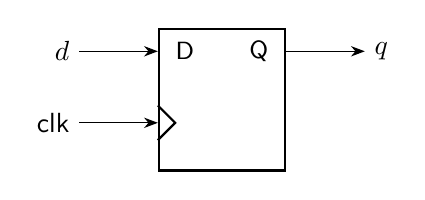
\begin{tikzpicture}[font=\sffamily]
  % flip-flop body
  \node[blk] (ff) {};
  % clock triangle on the left edge
  \draw[thick] ($(ff.south west)+(0,4mm)$) -- ++(2.2mm,2.2mm) -- ++(-2.2mm,2.2mm);
  % port labels inside
  \node[anchor=west, font=\sffamily\small] at ($(ff.north west)+(1mm,-3mm)$) {D};
  \node[anchor=east, font=\sffamily\small] at ($(ff.north east)+(-1mm,-3mm)$) {Q};
  % wires
  \draw[pin] ($(ff.north west)+(-10mm,-3mm)$) node[left]{$d$} -- ($(ff.north west)+(0,-3mm)$);
  \draw[pin] ($(ff.north east)+(0,-3mm)$) -- ++(10mm,0) node[right]{$q$};
  \draw[pin] ($(ff.south west)+(-10mm,6.2mm)$) node[left]{clk} -- ($(ff.south west)+(0,6.2mm)$);
\end{tikzpicture}
\end{document}
